\section{Results}

\subsection{Comparison of the deregulated pathwways in the PDCL with the TCGA-GBM datasets}

\subsubsection{Pathways mainly involved in the Cell-Cycle, DNA replication and Repair are shared between the two datasets}

The entry \textit{Glioma - Homo sapiens (human)} pathway (path:hsa05214) in \acrshort{kegg} document some of the deregulation caused by glioblastoma.
Zyla \textit{et al} used this entry as a target pathway to assess the sensitivity of different ranking metrics when studying microarray data from brain tissue \cite*{Zyla2017}.
\acrshort{fdr} value in G:Profiler is $8.898 \times 10^{-3}$ and $5.240 \times 10^{-2}$ respectively for \acrshort{pdcl} and \acrshort{tcga}, \acrshort{fdr} in \acrshort{gsea} is $4.487 \times 10^{-3}$ and $8.298 \times 10^{-1}$ respectively for \acrshort{pdcl} and \acrshort{tcga}.
Not only the \acrshort{fdr} value is lower for the \acrshort{tcga} dataset but the \acrshort{fdr} of \acrshort{gsea} for \acrshort{pdcl} does not pass the more lenient threshold we defined in this study.
Controls for the \acrshort{pdcl} dataset are taken from another study \cite*{Lundin2018}, this introduce variability not caused by deregulation of genes but more likely variability between samples or experimental conditions, while in the \acrshort{tcga} dataset controls comes from matching samples and follows the exact same protocol.
This might explain why the Glioma pathway is higher in the \acrshort{pdcl} dataset.

45 pathways are found deregulated in the \acrshort{pdcl} dataset and 304 in the \acrshort{tcga} dataset.
As can be seen in the figure \ref{fig:heatmap-fdr-global-tcga}, the two datasets shared 19 significantly deregulated pathways which are involved in the cell-cycle, DNA repair and replication, gene expression, extracellular matrix and in diseases.
\begin{figure}
    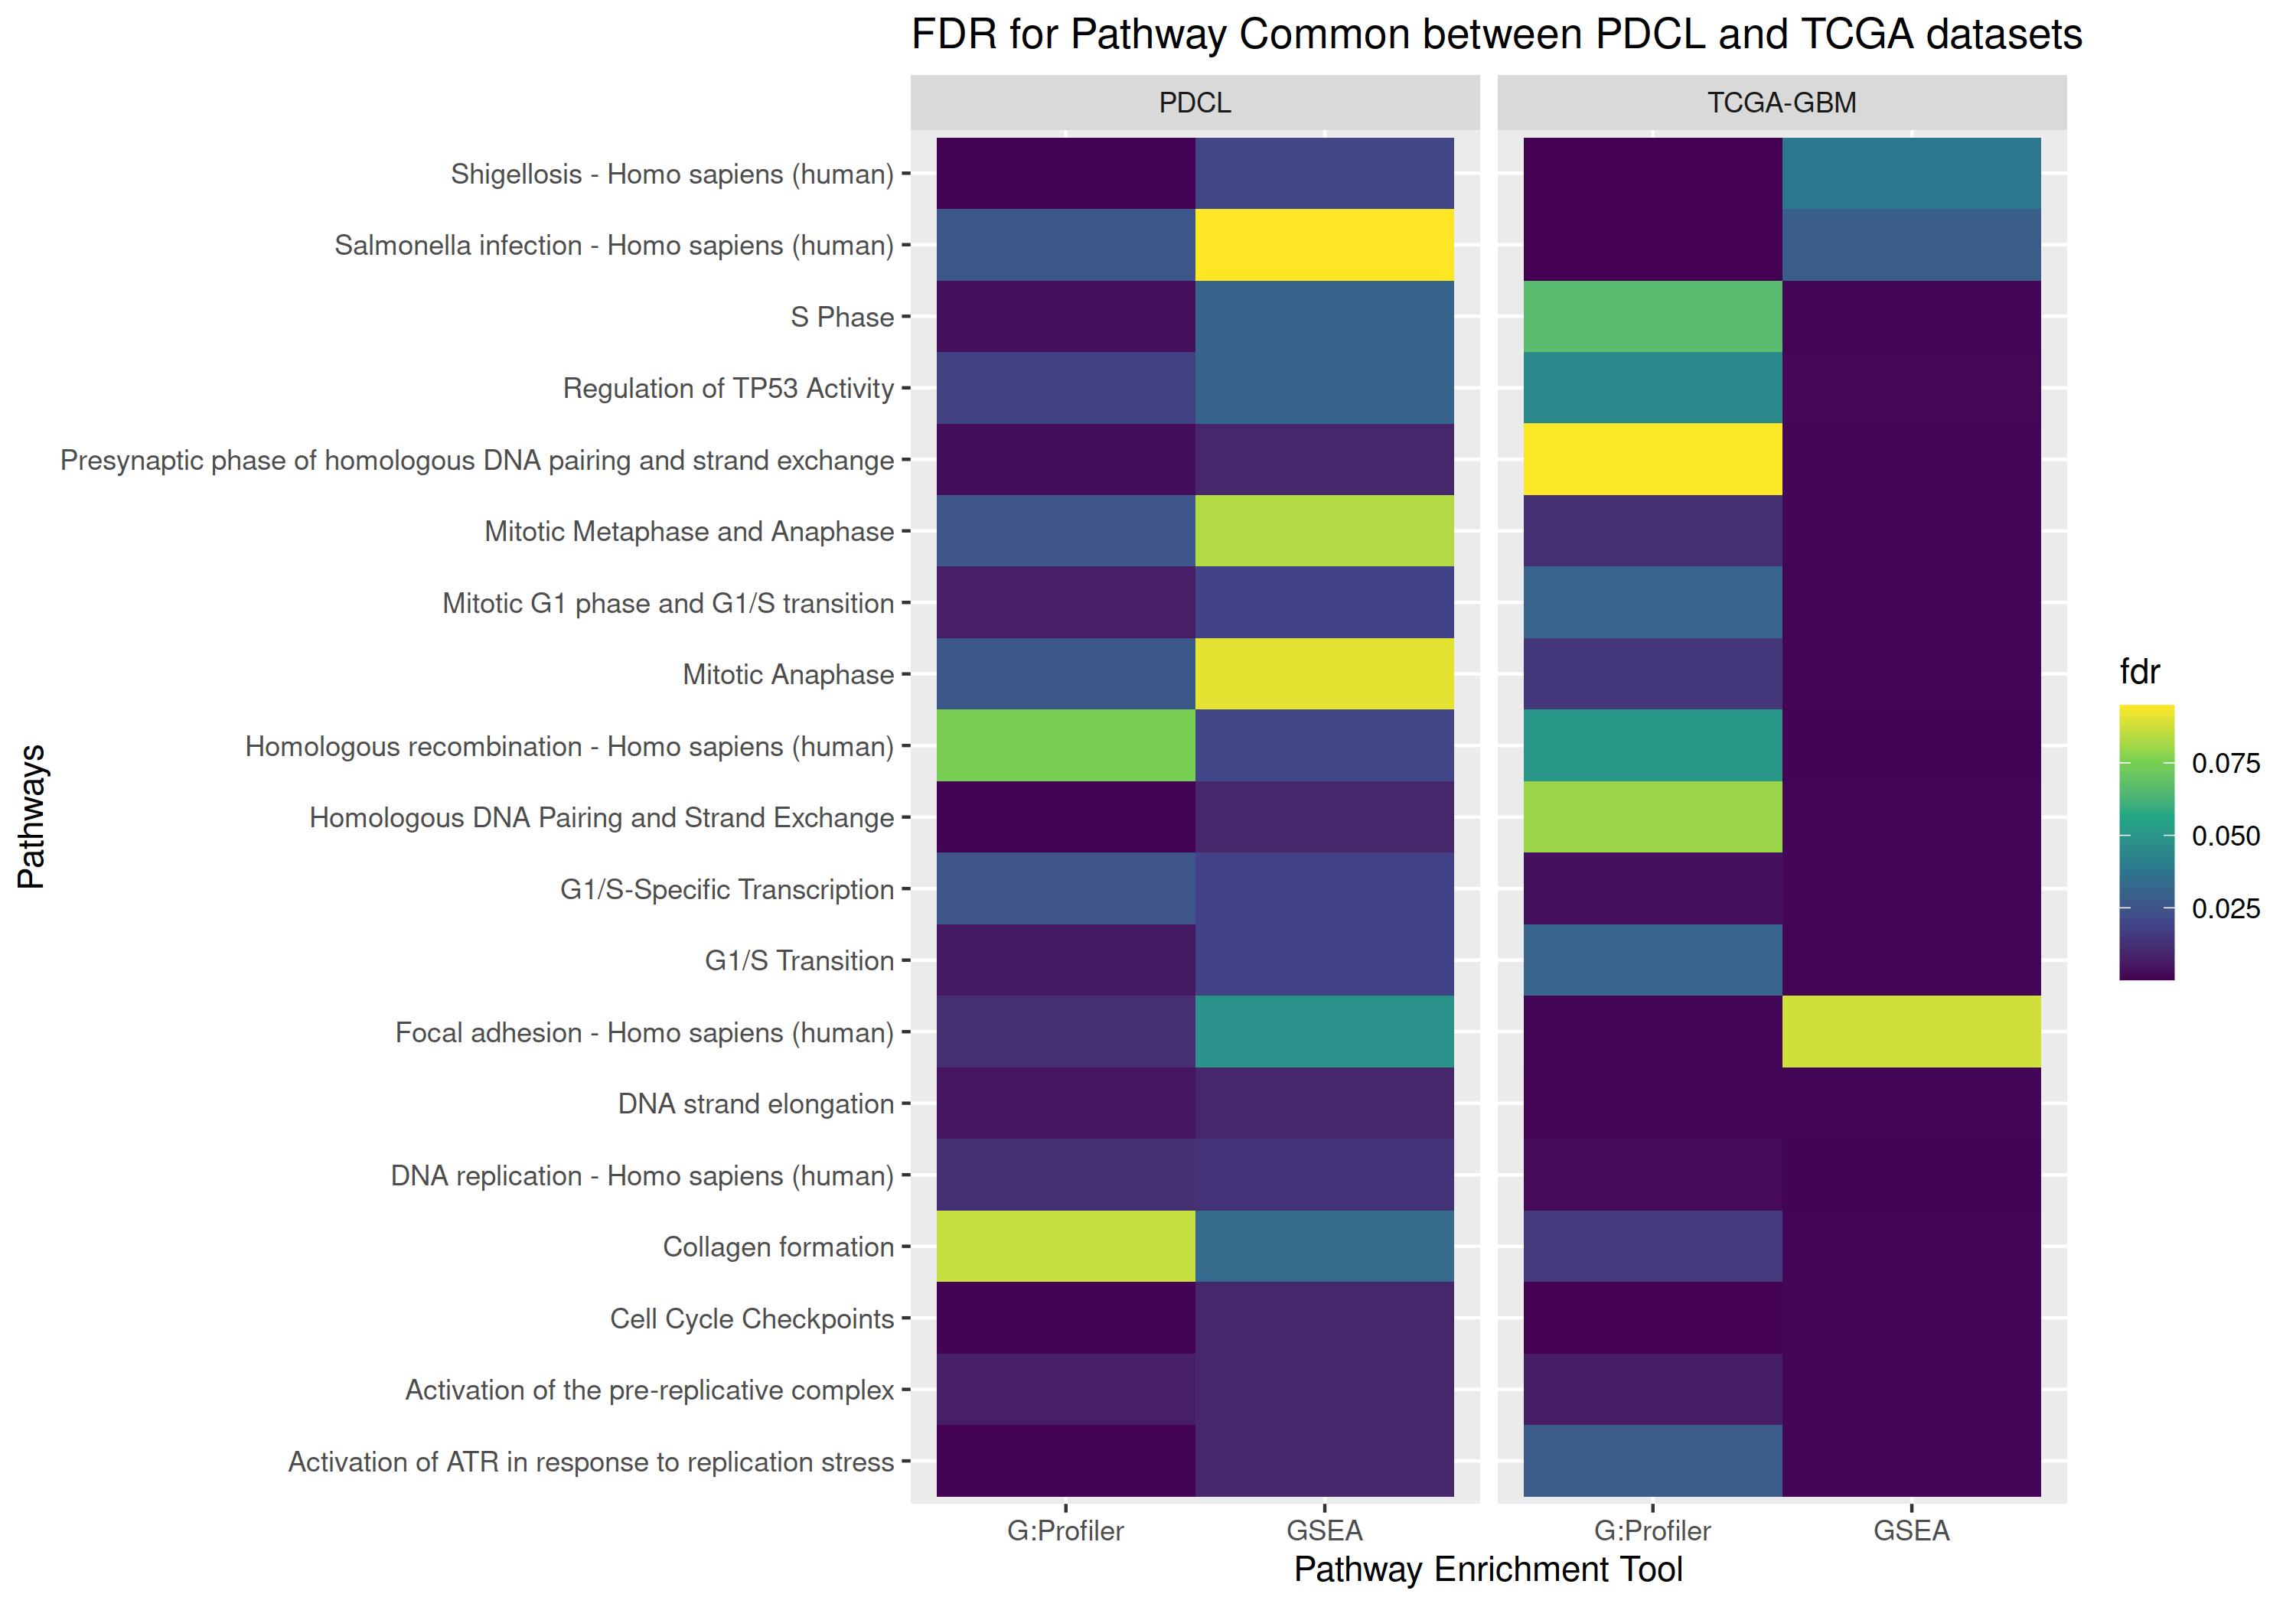
\includegraphics[width=\textwidth]{img/heatmap-fdr-global-tcga}
    \caption{
        \acrfull{fdr} of the pathways deregulated in both the \acrshort{pdcl} and the \acrshort{tcga} datasets.
        \acrshort{fdr} is lower than 0.1 since we only keep pathways that below this value.
    }
    \label{fig:heatmap-fdr-global-tcga}
\end{figure}
The 2 pathways associated with disease (Shigellosis and Salmonella infection) belong to the \acrshort{kegg} database.
However, pathways involved in DNA replication and repair are significantly enriched for both \acrshort{kegg} and Reactome.
Interestingly, the shared pathway \textit{Regulation of TP53 activity} is found upregulated by \acrshort{gsea} for both datasets.
A study from \acrshort{tcga} on frequent mutations in glioblastoma has showed that p53 signaling is altered  in 87\% of the samples and p53 is inactivated by mutation in 35\% of the samples \cite*{McLendon2008}.
Thus, regulation of p53 may be upregulated to make up for the lack of activity from the mutated p53.

Among the pathways enriched only in thez \acrshort{tcga} dataset, we found pathways that are children of the shared pathways between both dataset.
For example, \textit{Amplification of signal from unattached kinetochores via a MAD2 inhibitory signal} (R-HSA-141444) is a children pathway of \textit{Cell Cycle Checkpoints} (R-HSA-69620) that is to say it is smaller pathway which take place in its parent pathways.
When we compared the \acrshort{fdr} values of this pathways in G:Profiler and \acrshort{gsea} for both dataset, only G:Profiler's result does not pass the threshold used (\acrshort{fdr} value is 0.125 in G:Profiler with \acrshort{pdcl} sample).
Although almost all genes of this pathway are present in the dataset, closer look at the number of deregulated genes involved in this pathway in G:Profiler's result for both datasets showed 74 genes in the \acrshort{tcga} compared to 48 for \acrshort{pdcl}.
If we first hypothetized that the lower number of genes included in the \acrshort{pdcl} dataset (~20,000 genes compared to ~60,000 in \acrshort{tcga}) may reduce the ability of pathway enrichment tools to detect smaller pathways, this shows that it is rather caused the absence of deregulation in \acrshort{pdcl} samples.

\subsubsection{Cell-Cycle}

\subsubsection{Metabolism}

\subsubsection{Extra-Cellular Matrix}

\subsubsection{Neuronal System}

\subsection{Comparison of the deregulated pathways between PDCLs}

\subsubsection{ECM and Cholesterol biosynthesis among the most frequently deregulated pathways}

\subsubsection{PDCL samples exhibit different categories deregulated}

